\section{Background and Preliminary}
\label{sec:background}
UPRESSO is compatible with OIDC, and achieves the privacy protection based on the discrete logarithm problem.
Here, we provide a brief introduction on OIDC and the discrete logarithm problem.

\subsection{OpenID Connect}
\label{subsec:OIDC}
OIDC~\cite{OpenIDConnect} is an extension of OAuth 2.0 to support user authentication,
 and becomes one of the most prominent SSO authentication protocols.
Same as other SSO protocols~\cite{SAMLIdentifier}, OIDC involves three entities, i.e., {\em users}, {\em identity provider (IdP)}, and {\em relying parties (RPs)}.
Both users and RPs have to register at the IdP,    
the users register at the IdP to create credentials and identifiers (e.g. $ID_U$),
while each RP registers at the IdP with its endpoint information to create its unique identifier (e.g., $ID_{RP}$) and the corresponding credential.
IdP is assumed to securely maintain the attributes  of users and RPs.   
Then, in the SSO authentication sessions, 
 each user is responsible to start a login request at an RP, redirect the messages between RP and IdP, and check the scope of user's attributes provided to the RP;
 IdP authenticates the user, sets the $PPID$ for the user $ID_U$ at the RP $ID_{RP}$,
 constructs the identity proof with  $PPID$, $ID_{RP}$ and the user's attributes consented by the user, and finally transmits the identity proof to the RP's registered endpoint (e.g., URL);
 each RP constructs an identity proof request with its identifier and the requested scope of  user's attributes, sends an identity proof request to the IdP through the user, and parses the received identity proof to authenticate and authorize the user.
Usually, the redirection and checking at the user are handled by a user-controlled software, called {\em user agent} (e.g., browser).



\noindent\textbf{Implicit flow of user login.}
OIDC supports three processes for the SSO authentication session, known as {\em implicit flow}, {\em authorization code flow} and {\em hybrid flow} (i.e., a mix-up of the previous two).
In the implicit flow of OIDC, a token, known as {\em id token}, is introduced as the identity proof, which contains user identifier (i.e., $PPID$), RP identifier (i.e., $ID_{RP}$), the issuer (i.e., IdP), issuing time, the validity period, and other requested attributes. The IdP signs the id token using its private key to ensure integrity, and sends it through the user to RP.
In the authorization code flow, IdP binds an authorization code with the RP, and redirects this code to the RP;
 then RP establishes an HTTPS connection with IdP to ensure the integrity and confidentiality of the identity proof, and  uses the authorization code with the RP's credential to obtain PPID and the user's other  attributes.

UPRESSO is compatible to all the three flows.
For brevity, we will present the application of UPRESSO in the implicit flow in details, and provide the integration with the authorization code flow briefly. 
Here, we first introduce the original processes in the implicit flow of OIDC.
\begin{figure}[t]
  \centering
  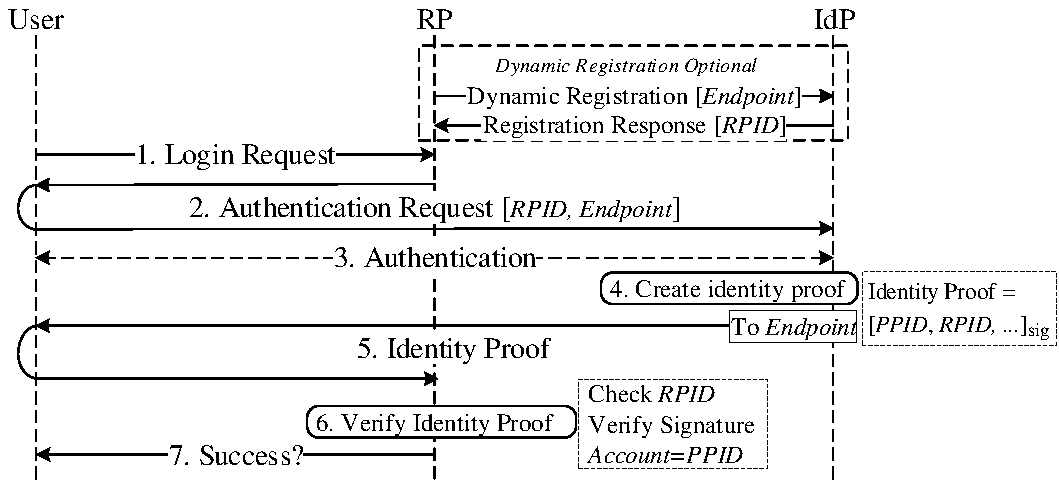
\includegraphics[width=\linewidth]{fig/OIDC1.pdf}
  \caption{The implicit protocol flow of OIDC.}
  \label{fig:OpenID}
\end{figure}
As shown in Figure~\ref{fig:OpenID}, the implicit flow of OIDC consists of 7 steps: when a user attempts to log in to an RP (Step 1), the RP constructs a request for identity proof, which is redirected by the user to the corresponding IdP (Step 2). The request contains $ID_{RP}$, RP's endpoint and a set of requested user attributes. If the user has not been authenticated yet, the IdP performs an authentication process (Step 3). If the RP's endpoint in the request matches the one registered at the IdP, it generates an identity proof (Step 4) and sends it back to the RP (Step 5). Otherwise, IdP generates a warning to notify the user about potential identity proof leakage. The RP verifies the id token (Step 6), extracts user identifier from the id token and returns the authentication result to the user (Step 7).



\begin{figure}[t]
  \centering
  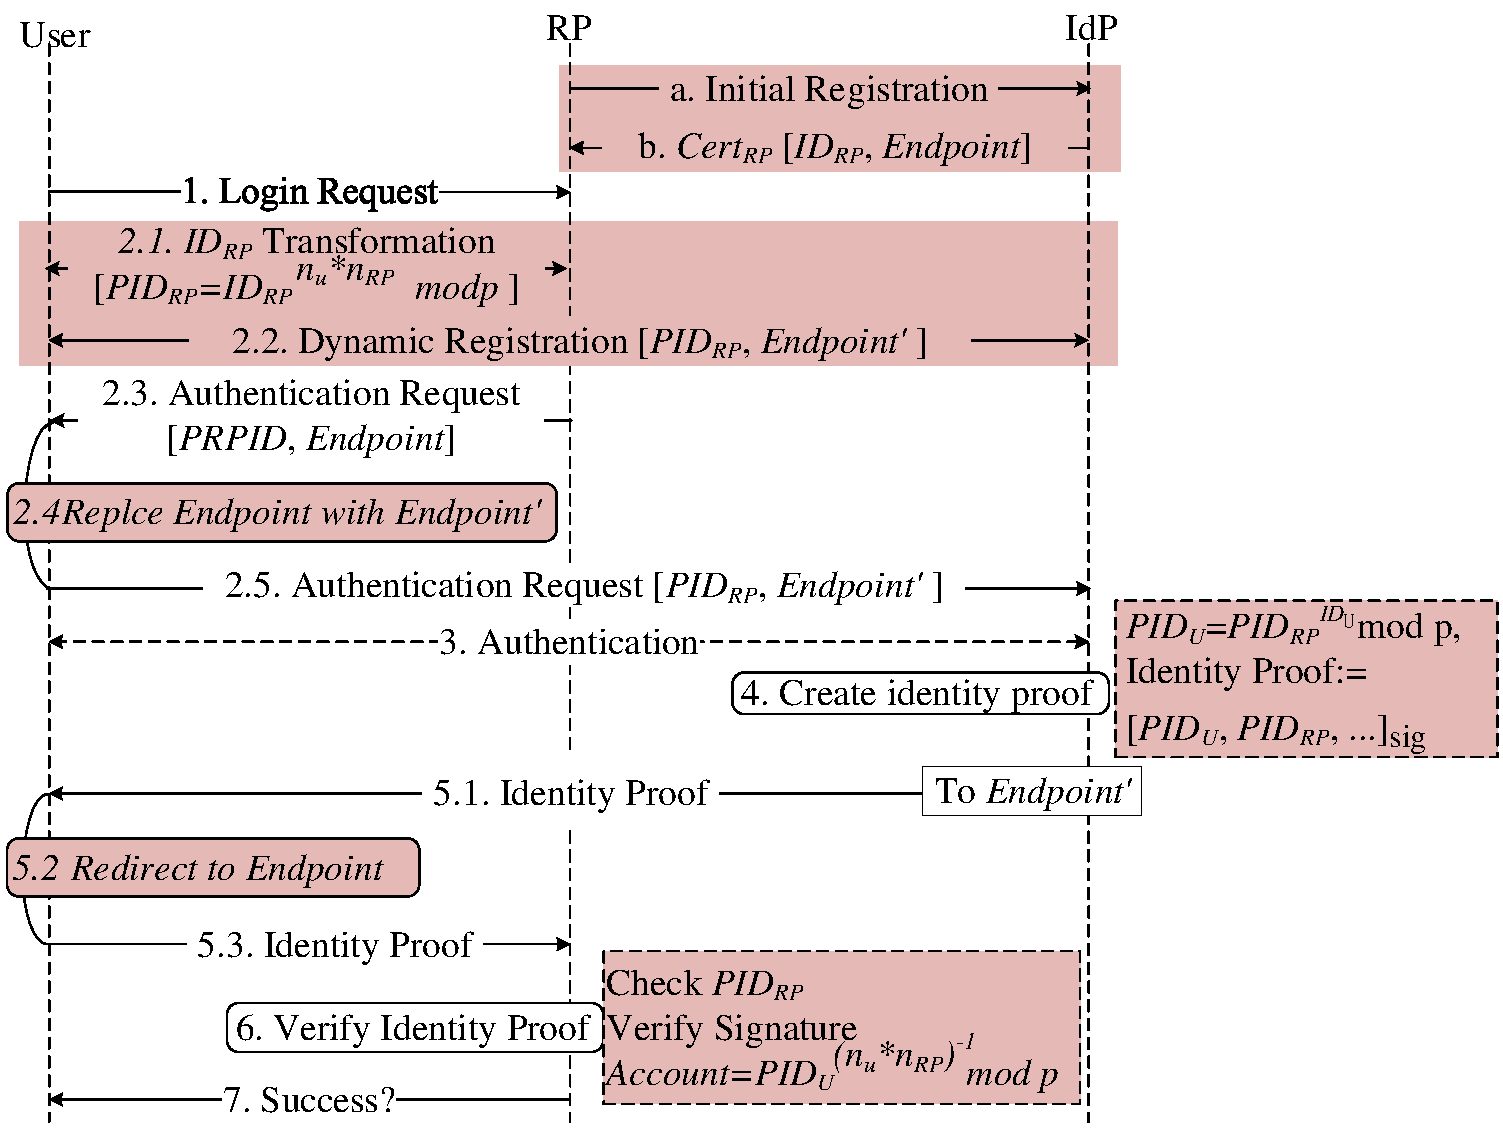
\includegraphics[width=\linewidth]{fig/overview1.pdf}
  \caption{The UPRESSO.}
  \label{fig:UPRESSO}
\end{figure}

\noindent\textbf{RP dynamic registration.} OIDC provides a dynamic registration mechanism~\cite{DynamicRegistration} for the RP to renew its $ID_{RP}$ dynamically. 
When an RP first registers at the IdP, it obtains a registration token, with which the  RP can invoke the dynamic registration process to
update its information (e.g., the endpoint). 
After each successful dynamic registration, the RP obtains a new unique $ID_{RP}$ from the IdP.
In UPRESSO, we slightly modify dynamic registration to register $PID_{RP}$ at IdP. 


\subsection{Discrete Logarithm Problem}
\label{sec:dlp}
Discrete logarithm problem is adopted in UPRESSO for the construction of $F_{PID_{RP}}$ and $F_{PID_U}$,
 which generate privacy-preserving user identifier (e.g. $PID_U$) and RP identifier (e.g. $PID_{RP}$) respectively.
Here, we provide a brief description of the discrete logarithm problem.

A number $g$ ($0<g<p$) is called a primitive root modular a prime $p$, if for ${\forall}y$ ($0<y<p$), there is a  number $x$ ($0\le x <p-1$) satisfying $y=g^x \pmod p$.
And, $x$ is called the discrete logarithm of $y$ modulo $p$. Given a large prime $p$, a primitive root $g$ and a number $y$, it is computationally infeasible to derive the discrete logarithm (here $x$) of $y$ (detailed in~\cite{WXWM}), which is called discrete logarithm problem.
The hardness of solving discrete logarithm has been used to construct several security primitives, including Diffie-Hellman key exchange and Digital Signature Algorithm (DSA).

In the process of $F_{PID_{RP}}$ and $F_{PID_U}$, we needs to calculate the primitive root for a  large prime $p$ as follows~\cite{Shoup,Wang}.
First, we retrieve a primitive root $g_m$  modulo $p$ from all the integers by finding the first integer passing  the primitive root checking.
 A lemma is propose to simply the checking, that if $p=2q+1$ ($q$ is a prime),  an integer $\mu \in (1, p-1)$ is a primitive root if and only if $\mu^2\neq 1 \ mod \ p$ and $\mu^q\neq 1 \ mod \ p$.
Then, based on $g_m$, we can calculate a new primitive root $g = g_{m}^{t} mod \ p$, where $t$ is an integer coprime to $p-1$.
 


